
%(BEGIN_QUESTION)
% Copyright 2006, Tony R. Kuphaldt, released under the Creative Commons Attribution License (v 1.0)
% This means you may do almost anything with this work of mine, so long as you give me proper credit

Hvordan kan følgende pneumatiske regulatormekanisme endres for å gjøre ``bias''-leddet justerbart?

$$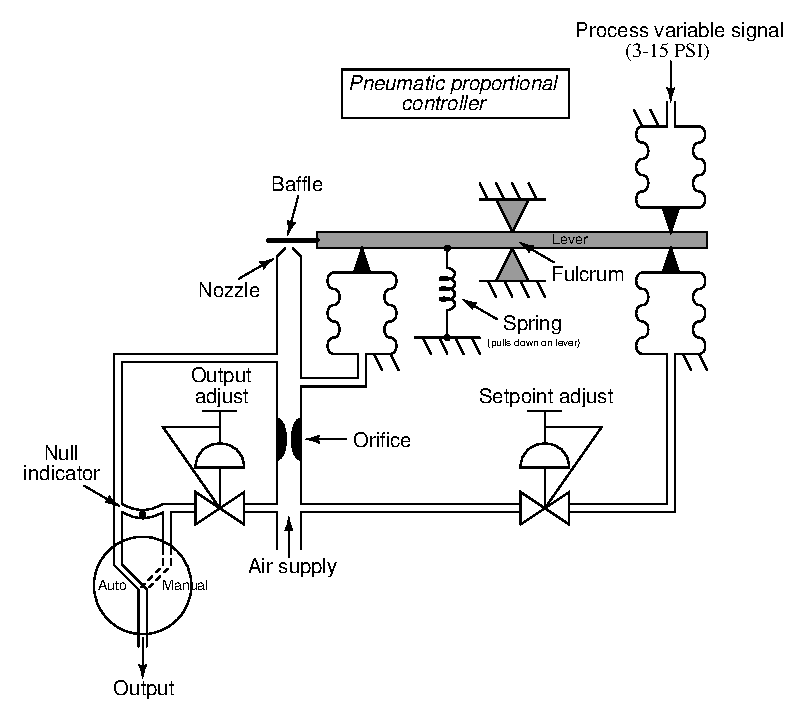
\includegraphics[width=15.5cm]{i01480x01.eps}$$

\underbar{file i01480}
%(END_QUESTION)





%(BEGIN_ANSWER)

$$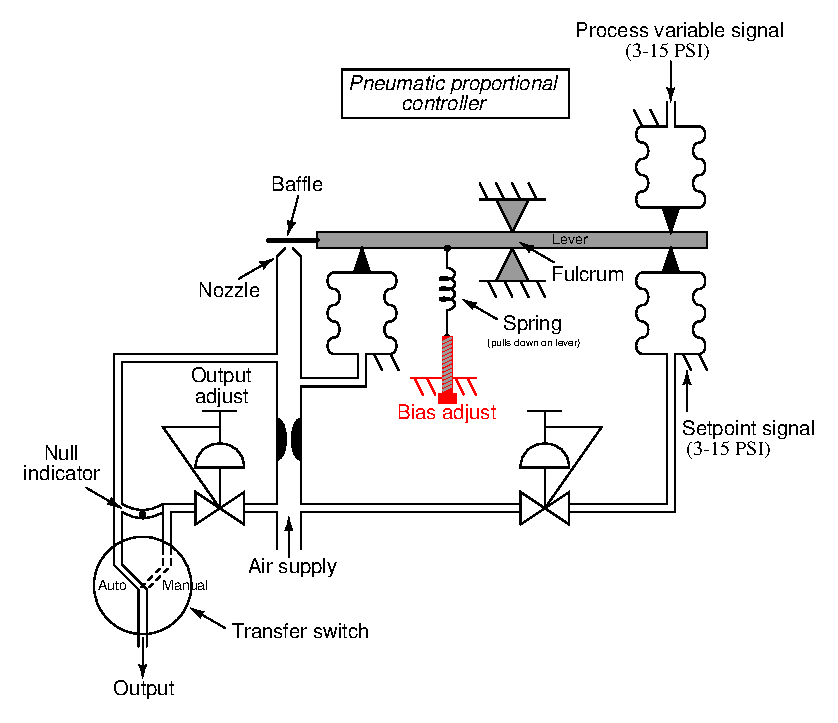
\includegraphics[width=15.5cm]{i01480x02.eps}$$

%(END_ANSWER)





%(BEGIN_NOTES)

Bias skapes av fjæren som trekker ned på armen. For å gjøre den justerbar kan fjærspenningen kobles til en skrue som kan flyttes. Minn studentene på at bias-leddet {\it legges til} den proporsjonale delen av regulatoren, og derfor må være en kraft som legges til (eller trekkes fra) kreftene i kraftbalansesystemet.

%INDEX% Control, proportional: pneumatic controller bias adjustment

%(END_NOTES)

